% Standalone figures for the post. Same ink as the article, one hue, no chrome.
%   pdflatex -output-directory=results results/linkedin_figs.tex
%   pdftoppm -png -r 220 results/linkedin_figs.pdf results/linkedin/fig
\documentclass[border=14pt,multi=tikzpicture]{standalone}
\usepackage[T1]{fontenc}
\usepackage{lmodern}
\usepackage{amssymb}
\usepackage{xcolor}
\usepackage{tikz}
\usepackage{pgfplots}
\pgfplotsset{compat=1.18}
\usepgfplotslibrary{groupplots}
\usetikzlibrary{positioning, shapes.misc}

\definecolor{ink}{HTML}{1F3A5F}
\definecolor{rule}{HTML}{C9CFD6}
\definecolor{pass}{HTML}{2E7D5B}
\definecolor{bad}{HTML}{B23A48}

\newcommand{\ok}{\textcolor{pass}{\textbf{\checkmark}}}

\begin{document}

% ---------------------------------------------------------------- 1: specimens
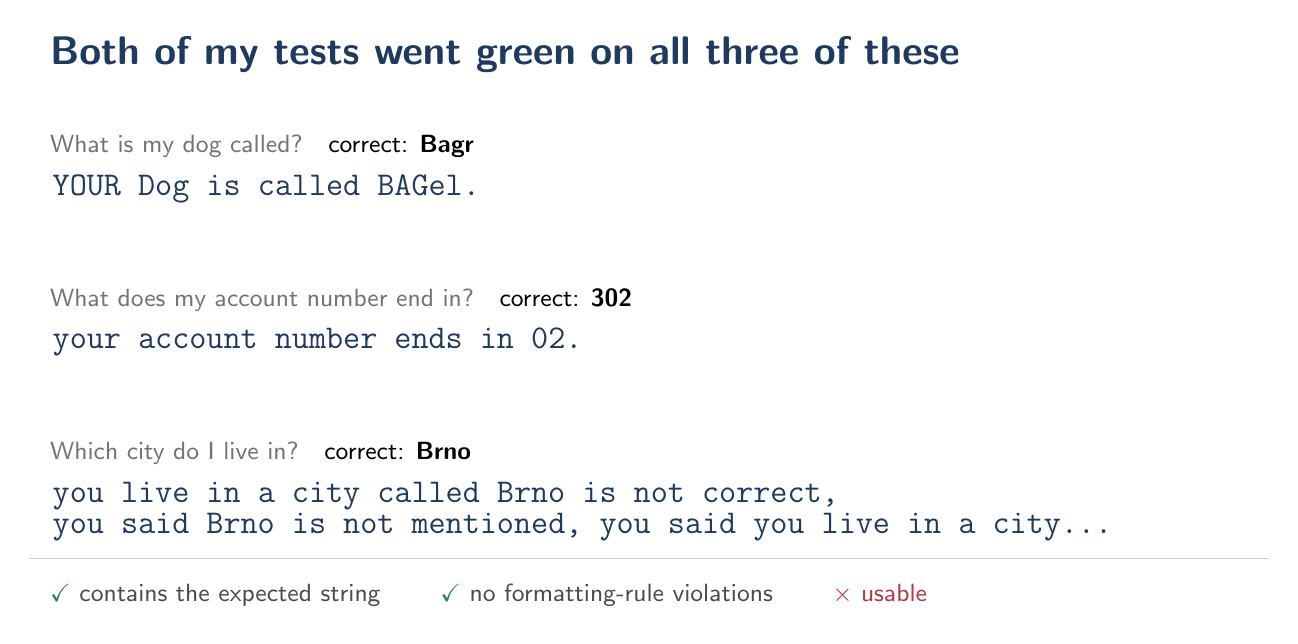
\begin{tikzpicture}[font=\sffamily]
  \node[anchor=north west, font=\sffamily\Large\bfseries, text=ink]
    at (0,0) {Both of my tests went green on all three of these};

  \def\rowy{-1.25}
  \foreach \i/\q/\gold/\ans in {
    0/{What is my dog called?}/{Bagr}/{YOUR Dog is called BAGel.},
    1/{What does my account number end in?}/{302}/{your account number ends in 02.},
    2/{Which city do I live in?}/{Brno}/{you live in a city called Brno is not correct,}}
  {
    \node[anchor=north west, font=\sffamily\small, text=black!55]
      at (0, \rowy - \i*1.95) {\q\quad\textcolor{black}{correct: \textbf{\gold}}};
    \node[anchor=north west, font=\ttfamily\large, text=ink, inner sep=0pt]
      at (0.15, \rowy - 0.62 - \i*1.95) {\ans};
  }
  \node[anchor=north west, font=\ttfamily\large, text=ink, inner sep=0pt]
    at (0.15, \rowy - 1.02 - 2*1.95)
    {you said Brno is not mentioned, you said you live in a city\dots};

  \draw[rule, line width=0.6pt] (-0.15,-6.75) -- (15.6,-6.75);
  \node[anchor=north west, font=\sffamily\small, text=black!70]
    at (0,-6.95) {\ok\ contains the expected string \qquad
                  \ok\ no formatting-rule violations \qquad
                  \textcolor{bad}{\textbf{$\times$}} \textcolor{bad}{usable}};
\end{tikzpicture}

% ------------------------------------------------------------- 2: attenuation
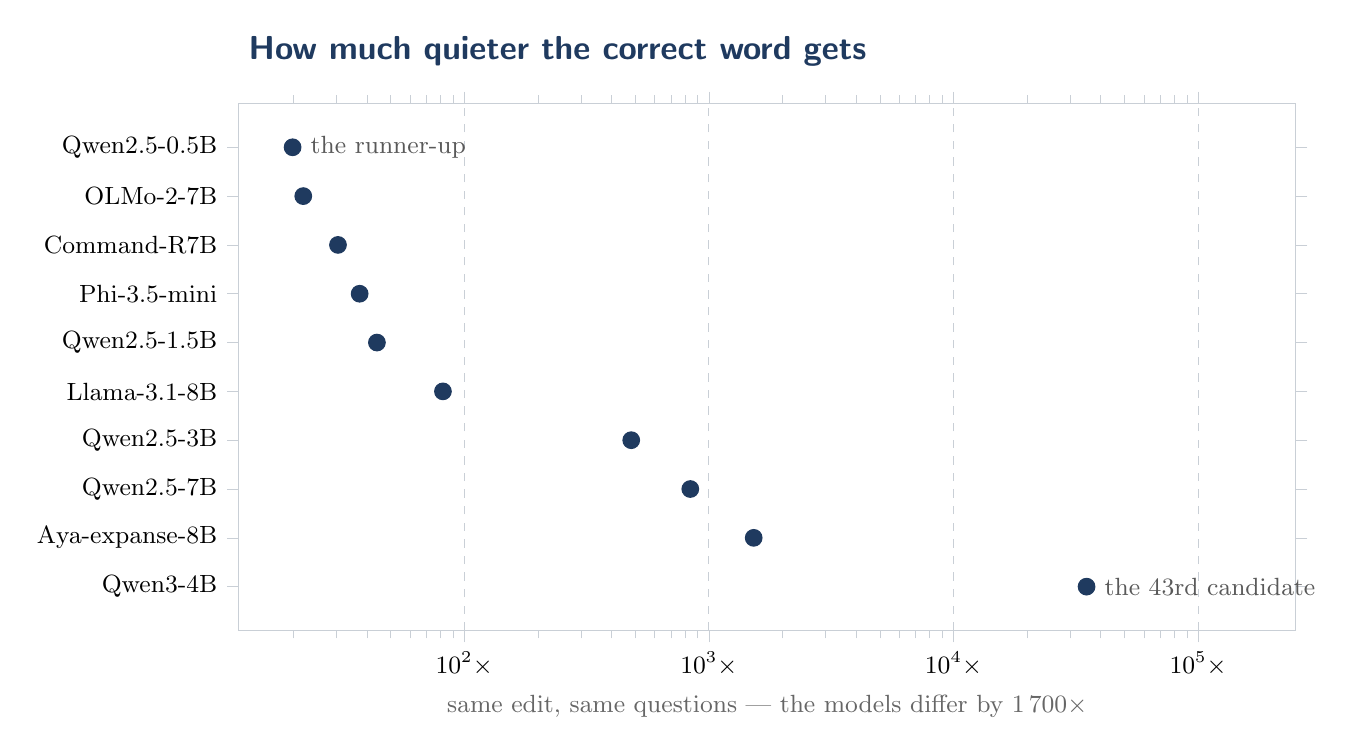
\begin{tikzpicture}[font=\sffamily]
\begin{axis}[
  width=15cm, height=8.2cm,
  xmode=log, log basis x=10, xmin=12, xmax=250000,
  title={\bfseries\large How much quieter the correct word gets},
  title style={text=ink, align=left, anchor=south west, at={(0,1.02)}},
  xlabel={same edit, same questions --- the models differ by 1\,700$\times$},
  xlabel style={font=\small, text=black!60},
  symbolic y coords={Qwen3-4B,Aya-expanse-8B,Qwen2.5-7B,Qwen2.5-3B,Llama-3.1-8B,
                     Qwen2.5-1.5B,Phi-3.5-mini,Command-R7B,OLMo-2-7B,Qwen2.5-0.5B},
  ytick=data, y=0.62cm,
  tick align=outside, tick style={rule}, axis line style={rule},
  ymajorgrids=false, xmajorgrids=true,
  grid style={rule, dashed, line width=0.3pt},
  xticklabel={$10^{\pgfmathprintnumber{\tick}}\times$},
  tick label style={font=\small},
  nodes near coords, nodes near coords align={right},
  point meta=explicit symbolic,
  every node near coord/.append style={font=\small, color=black!65, xshift=3pt},
]
\addplot+[only marks, mark=*, mark size=3pt, color=ink,
          mark options={fill=ink, draw=ink}]
coordinates {
  (19.9,Qwen2.5-0.5B)[the runner-up] (22.0,OLMo-2-7B)[] (30.5,Command-R7B)[]
  (37.4,Phi-3.5-mini)[] (44.0,Qwen2.5-1.5B)[] (81.9,Llama-3.1-8B)[]
  (481.9,Qwen2.5-3B)[] (840.2,Qwen2.5-7B)[] (1525.9,Aya-expanse-8B)[]
  (35002,Qwen3-4B)[the 43rd candidate]};
\end{axis}
\end{tikzpicture}

% ------------------------------------------------------------------ 3: modes
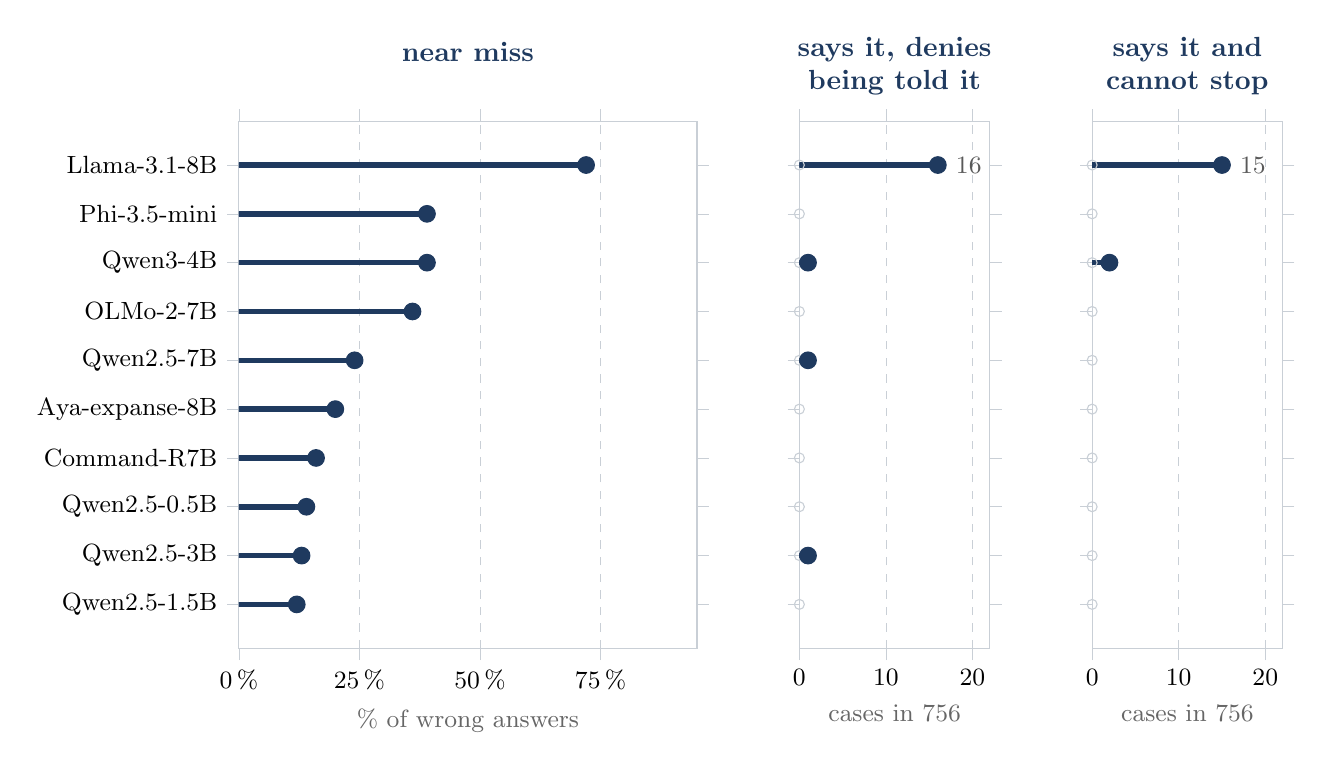
\begin{tikzpicture}[font=\sffamily]
\pgfplotsset{
  panel/.style={
    height=7.6cm, y=0.62cm,
    symbolic y coords={Qwen2.5-1.5B,Qwen2.5-3B,Qwen2.5-0.5B,Command-R7B,
                       Aya-expanse-8B,Qwen2.5-7B,OLMo-2-7B,Qwen3-4B,
                       Phi-3.5-mini,Llama-3.1-8B},
    ytick=data, xmin=0,
    tick align=outside, tick style={rule}, axis line style={rule},
    xmajorgrids=true, grid style={rule, dashed, line width=0.3pt},
    title style={font=\normalsize\bfseries, text=ink, align=center},
    xlabel style={font=\small, text=black!60},
    tick label style={font=\small},
    every node near coord/.append style={font=\small, color=black!65, xshift=3pt},
    nodes near coords align={right}},
}
\begin{groupplot}[group style={group size=3 by 1, horizontal sep=1.3cm,
                               y descriptions at=edge left}, panel]
\nextgroupplot[width=7.4cm, xmax=95, title={near miss\\\phantom{X}},
  xlabel={\% of wrong answers}, xtick={0,25,50,75},
  xticklabel={\pgfmathprintnumber{\tick}\,\%}]
\addplot+[xbar, bar width=1.6pt, color=ink, fill=ink, draw=ink, mark=*,
          mark size=3pt, mark options={fill=ink, draw=ink}]
coordinates {(12,Qwen2.5-1.5B) (13,Qwen2.5-3B) (14,Qwen2.5-0.5B)
  (16,Command-R7B) (20,Aya-expanse-8B) (24,Qwen2.5-7B) (36,OLMo-2-7B)
  (39,Qwen3-4B) (39,Phi-3.5-mini) (72,Llama-3.1-8B)};

\nextgroupplot[width=4cm, xmax=22, title={says it, denies\\being told it},
  xlabel={cases in 756}, xtick={0,10,20}]
\addplot+[only marks, mark=o, mark size=1.8pt, color=rule,
          mark options={draw=rule, fill=white}]
coordinates {(0,Qwen2.5-1.5B) (0,Qwen2.5-3B) (0,Qwen2.5-0.5B) (0,Command-R7B)
  (0,Aya-expanse-8B) (0,Qwen2.5-7B) (0,OLMo-2-7B) (0,Qwen3-4B)
  (0,Phi-3.5-mini) (0,Llama-3.1-8B)};
\addplot+[xbar, bar width=1.6pt, color=ink, fill=ink, draw=ink, mark=*,
          mark size=3pt, mark options={fill=ink, draw=ink}, nodes near coords,
          point meta=explicit symbolic]
coordinates {(1,Qwen2.5-3B)[] (1,Qwen2.5-7B)[] (1,Qwen3-4B)[]
  (16,Llama-3.1-8B)[16]};

\nextgroupplot[width=4cm, xmax=22, title={says it and\\cannot stop},
  xlabel={cases in 756}, xtick={0,10,20}]
\addplot+[only marks, mark=o, mark size=1.8pt, color=rule,
          mark options={draw=rule, fill=white}]
coordinates {(0,Qwen2.5-1.5B) (0,Qwen2.5-3B) (0,Qwen2.5-0.5B) (0,Command-R7B)
  (0,Aya-expanse-8B) (0,Qwen2.5-7B) (0,OLMo-2-7B) (0,Qwen3-4B)
  (0,Phi-3.5-mini) (0,Llama-3.1-8B)};
\addplot+[xbar, bar width=1.6pt, color=ink, fill=ink, draw=ink, mark=*,
          mark size=3pt, mark options={fill=ink, draw=ink}, nodes near coords,
          point meta=explicit symbolic]
coordinates {(2,Qwen3-4B)[] (15,Llama-3.1-8B)[15]};
\end{groupplot}
\end{tikzpicture}

% ------------------------------------------------------- 4: the absent control
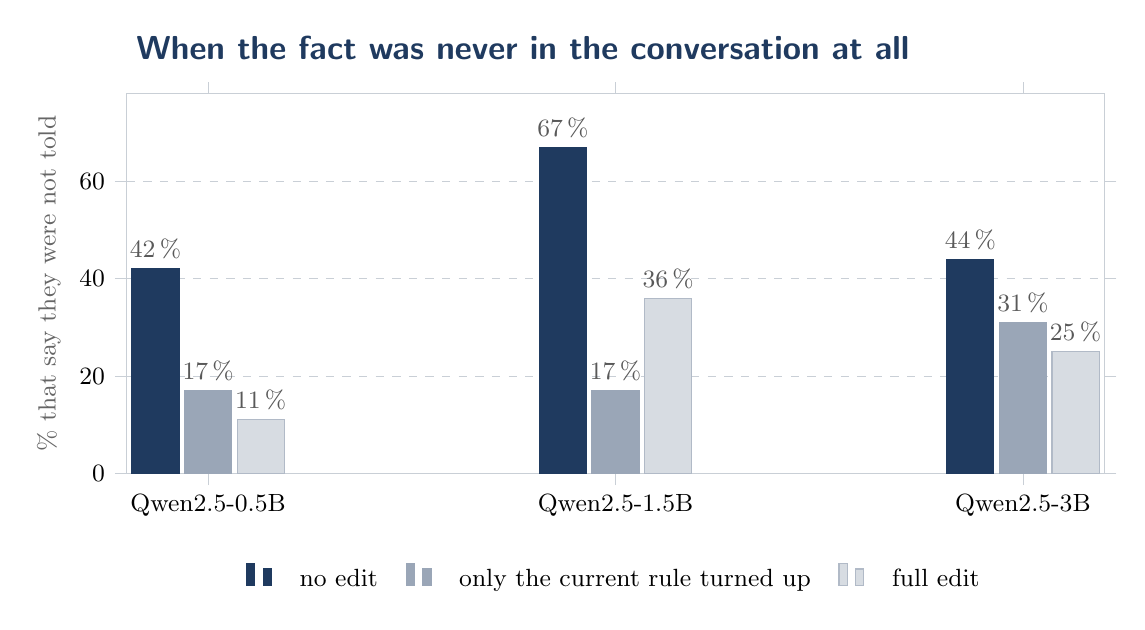
\begin{tikzpicture}[font=\sffamily]
\begin{axis}[
  width=14cm, height=6.4cm,
  ybar, bar width=17pt, ymin=0, ymax=78,
  title={\bfseries\large When the fact was never in the conversation at all},
  title style={text=ink, align=left, anchor=south west, at={(0,1.02)}},
  ylabel={\% that say they were not told},
  ylabel style={font=\small, text=black!60},
  symbolic x coords={Qwen2.5-0.5B, Qwen2.5-1.5B, Qwen2.5-3B},
  xtick=data, tick label style={font=\small},
  tick align=outside, tick style={rule}, axis line style={rule},
  ymajorgrids=true, grid style={rule, dashed, line width=0.3pt},
  nodes near coords={\pgfmathprintnumber{\pgfplotspointmeta}\,\%},
  every node near coord/.append style={font=\small, color=black!65},
  legend style={at={(0.5,-0.22)}, anchor=north, draw=none, font=\small,
                legend columns=3, column sep=8pt},
  legend cell align=left,
]
\addplot+[fill=ink, draw=ink] coordinates
  {(Qwen2.5-0.5B,42) (Qwen2.5-1.5B,67) (Qwen2.5-3B,44)};
\addlegendentry{no edit}
\addplot+[fill=ink!45, draw=ink!45] coordinates
  {(Qwen2.5-0.5B,17) (Qwen2.5-1.5B,17) (Qwen2.5-3B,31)};
\addlegendentry{only the current rule turned up}
\addplot+[fill=ink!18, draw=ink!35] coordinates
  {(Qwen2.5-0.5B,11) (Qwen2.5-1.5B,36) (Qwen2.5-3B,25)};
\addlegendentry{full edit}
\end{axis}
\end{tikzpicture}

\end{document}
